\graphicspath{{fig/scoters/}}

\chapter{Case Study II: foraging scoters}
\label{cha:scoters}

In the previous chapter we discussed how the use of fixed-location recording
equipment during data acquisition can result in individuals moving out-of-frame
\emph{during} recording. Such movements are then missing from the recorded
flocking event. As out-of-frame movement may still be influencing the behaviour
of the observed flock, this movement must be accounted for during model
fitting. In \cref{cha:missing} we demonstrated methodology to account for such
missingness in \emph{simulated} data. In this chapter we consider a \emph{real}
flocking event with missing observations. As foreshadowed in the previous
chapter, the missing observations of this dataset will be realised as a
consequence of employing fixed-location recording equipment.

The dataset considered in this chapter describes the movements of a large
number of surf scoters, a migratory sea bird, which gather in groups to forage.
The captured flocking events take place on the surface of a lake, and so
movement is effectively restricted to a two-dimensional plane. This dataset was
provided courtesy of work performed by \textcite{lukeman09,lukeman10}. At the
time of their publication the captured events represented a tenfold increase in
the number of individuals which could be reliably linked \emph{between} frames.

Unfortunately, owing to the fixed-location cameras used to record these
flocking events, there were often scoters out of view in the recorded frames.
\cref{fig:lukeman_extraction} illustrates the steps performed to extract the
positions of individuals from raw footage; this figure also shows how the flock
occupied an area larger than that which the camera captured---resulting in
missing observations. As in \cref{cha:missing}, the missing data points can be
partitioned into observations missing at the \emph{beginning} of the recording
event, and observations missing at the \emph{end} of the recording event.

In this chapter we shall fit a simple variation of the Vicsek model to a
flocking event of the Lukeman dataset. The missing observations will be
integrated out of the problem using methodology developed in
\cref{cha:missing}.

\section{Scoter data}

\textcite{lukeman10} recorded a number of flocking events from an aerial
vantage point: an elevated promenade at the side of a large lake. From this
position the authors were able to direct a camera toward an inlet where
overwintering scoters had been observed foraging. Knowing the height of this
camera above the water, and the angle of its approach with the horizontal, the
authors were able to transform the captured camera data back to ``real-world''
co-ordinates.

However, to reliably transform back from camera co-ordinates to real-world
co-ordinates, the height of the camera above the lake and its angle with the
horizontal had to be fixed. With the camera fixed in position, the authors then
waited for flocking events to occur. Recording began when individuals entered
the camera's field of vision, and ended when all the individuals left the
frame, or the flock became stationary. Each recording event captured the
movements of around $170$ scoters, with each event consisting of approximately
$30$ frames. However, of the recorded events between $16\%$ and $64\%$ of each
flock's movements took place out-of-frame.

\textcite{lukeman10} discounted the influence of individuals out-of-frame, and
instead focused on reproducing radial and angular neighbour distributions of
\emph{internal} group members (edge individuals were also discarded). This
approach, although representing a significant step forward in the literature,
came with its drawbacks. Most significantly, focusing the fitting on
reproducing radial and angular neighbour distributions removed the
\emph{dynamic} component to the data which the authors worked so hard to
achieve. Additionally, the authors determined the size of the agents'
interaction radius by visual inspection of nearest-neighbour densities; the
interaction radius used in their model being chosen \emph{before} the fitting
process began.

In this chapter we take a more holistic approach to model fitting; making sure
to account for \emph{all} individuals---both observed and missing, as well as
internal and boundary individuals---and focusing the fitting on reproducing
the \emph{movements} of the flock, rather than some epiphenomena of their
movements. Significant computation is necessary to account for the large amount
of data missing from the recorded flocking events.

\section{Performing inference}

In \cref{cha:missing} we discussed how the computational demands of missing
data problems increase as the amount of missingness increases. With this in
mind we focus on the flocking event within the Lukeman dataset which displays
the \emph{least} amount of missingness. For the events captured by
\textcite{lukeman10} this is represented by a sequence of $199$ scoters moving
over $23$ frames. Of the $199\times23=4577$ data points represented by this
event, $680$ ($\approx16\%)$ occur outside the visual field of the camera. This
flock is visualised in \cref{fig:scoter_traj}. From this figure we see that the
flock was strongly polarised throughout the recording event; with this
observation we consider an alignment-based model a plausible candidate model
for fitting.

\begin{figure}[tb]
  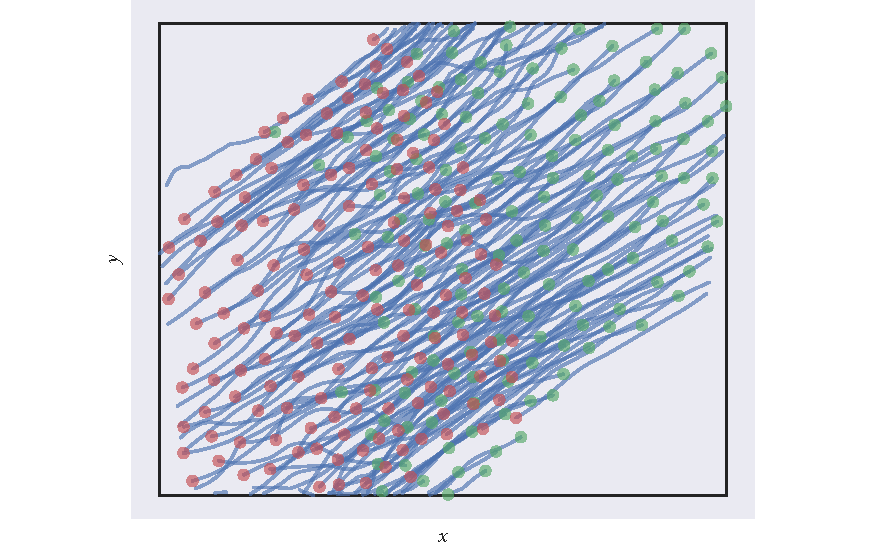
\includegraphics{data_00_traj.pdf}
  \caption{A visualisation of the trajectories of foraging surf scoters in an
    analysed sequence. In total the sequence represents the movements of
    $199$ scoters over $23$ frames ($4577$ data points). The scoters move
    along the blue trajectories, starting from the positions denoted by the
    green markers and finishing at the positions shown by the red markers. The
    black frame containing the trajectories represents an approximation of the
    fixed field of vision of the recording equipment.}
  \label{fig:scoter_traj}
\end{figure}

\cref{fig:scoter_missing} gives a visual representation of which data points
were observed, and which data points were missing. In this visualisation blue
markers represent observed data and red markers represent missing data. From
\cref{fig:scoter_missing} we see that in \emph{every frame} there is \emph{at
least one} missing scoter. As such, if we were to discard all the frames with
as least one missing scoter (as in the naive approach outlined in
\cref{cha:missing}), we would discard the entire flocking event. Therefore to
evaluate the likelihood of observing this flock we have no choice but to
account for the missing observations.

The simulated flocks considered in \cref{cha:missing} had between $10$ and $20$
missing observations per sequence. With $680$ data points missing from the
scoter sequence with the \emph{least} amount of missingness, this problem
represents a considerable increase in complexity. With this amount of
missingness, long and expensive simulations were necessary to realise a
satisfactory number of samples from the posterior.

\begin{figure}[tb]
  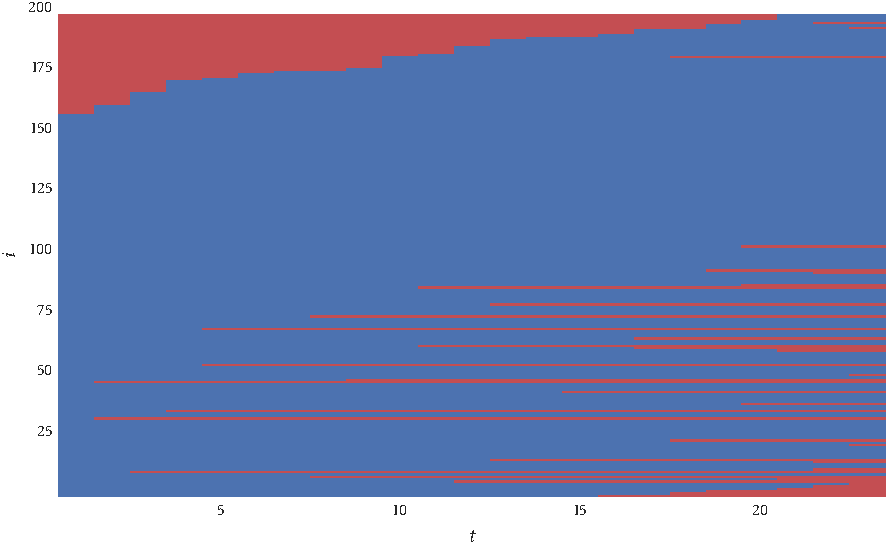
\includegraphics{data_00_missing.pdf}
  \caption{A representation of the missing and observed data points of the
    foraging event illustrated in \cref{fig:scoter_traj}. The $x$-axis
    represents the frame of the sequence, and the $y$-axis corresponds to
    tracked individuals. A blue tile at location $(t, i)$ tells us that scoter
    $i$ was observed in frame $t$. A red tile at location $(t, i)$ indicates
    that scoter $i$ was missing at time $t$.}
  \label{fig:scoter_missing}
\end{figure}

We fit a variation of the Vicsek model to this dataset where each agent
interacts with neighbours within distance $r$ (\cref{eq:vicsek_interaction}),
and experiences noise sampled from a generalised Student's $t$ distribution
with $\nu$ degrees of freedom and scale $\sigma_Y$ (\cref{eq:students_update}).
A random walk Metropolis--Hastings algorithm was implemented to infer the
parameters of this model. In a similar manner, a random walk
Metropolis--Hastings algorithm, with proposal scheme as outlined in
\cref{ssec:beg_missing}, was used to infer the observations missing at the
beginning of the sequence. Finally, using a Gibbs step allowed observations
missing at the end of the sequence to be sampled. This sampler was implemented
for $10^8$ iterations. To reduce the memory overhead of this sampler, the
recorded samples were thinned by a factor of $1000$; meaning that all but every
$1000$-th iteration of the sampler was discarded, producing a total of $10^8 /
10^3 = 10^5$ samples.

In \cref{cha:missing} we used summary plots---such as those in
\cref{fig:beg_summary,fig:end_summary}---to help visualise high-dimensional
posterior distributions. However, with almost $700$ dimensions, this posterior
has too many dimensions for even these summary plots. In such a situation it
can be informative to graphically assess the trace of the log-likelihood. If we
can observe that the log-likelihood has converged, we have good evidence that
the sampler has converged. In \cref{fig:log_ll} we see a trace and histogram
plot of evaluations of the log-likelihood. From this plot we see evidence of
convergence, as the log-likelihood oscillates regularly around some fixed
location.

\begin{figure}[tb]
  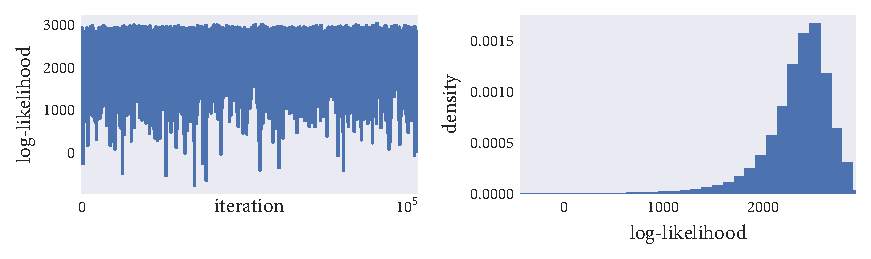
\includegraphics{log_likelihood.pdf}
  \caption{Trace and histogram plots of the log-likelihood, as computed at
    every iteration of the inference scheme. As it can be difficult to assess
    the convergence of all the parameters for high-dimensional problems, as
    we have here, it can instead be informative to assess the convergence of
    the log-likelihood. If we see that the value of the log-likelihood has
    converged, then we have evidence that the chains targeting the corresponding
    parameters also converged.}
    \label{fig:log_ll}
\end{figure}

The parameters of the Vicsek model inferred in this fitting are shown in
\cref{fig:lukeman_params}. The tendency of the interaction radius $r$ towards
zero suggests that there is no direct alignment interaction between individuals
of this flock. The flock's highly polarised structure must then be the result
of behaviours unaccounted for by our model: such as attraction or repulsion
interactions. With no effective interaction term, all observed directional
changes must be accounted for by the inferred noise parameters, as in the Null
model (\cref{sec:null_model}). The inferred degrees of freedom and noise-scale
parameters represent a diffuse noise distribution, reflecting their need to
capture all directional changes.

\begin{figure}[tb]
  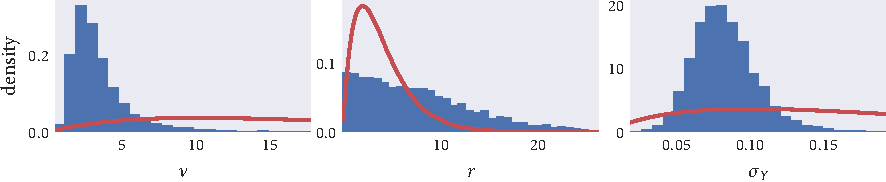
\includegraphics{params_hist.pdf}
  \caption{Samples drawn from the posterior distribution realised in fitting a
    sequence of the Lukeman data to a variation of the Vicsek model. The
    posterior distribution of $r$ is non-normal, and tends towards zero,
    representing evidence that there is no explicit alignment interaction
    between individuals.}
  \label{fig:lukeman_params}
\end{figure}

In \cref{fig:dir_hist} we see histogram plots of samples realised from the
posterior: here representing four directions missing at the end of the
sequence. We see that the uncertainty in the possible directions of motion of
the missing agent is large. This large posterior variance is a result of the
large amounts of missingness. As no effective interaction term was realised, a
diffuse noise structure was inferred to account for the observed directional
changes. This diffuse noise structure further contributes to the large
posterior variance inferred for the missing directions.

Although our model has been unable to capture the interactions between
individuals present in this flock, it is only by handling the missing data that
we have been able to fit this model and make this realisation.

\begin{figure}[tb]
  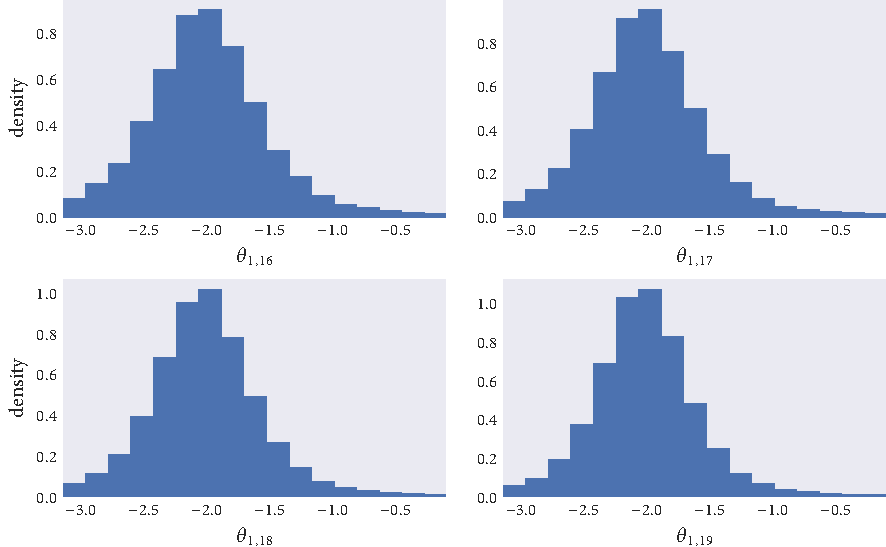
\includegraphics{dir_hist.pdf}
  \caption{Histogram plots of posterior draws of $4$ missing directions (out of
    a total of $680$ missing data points). The posterior draws visualised
    correspond to data missing at the end of the sequence. We see large amounts
    of uncertainty in these posterior densities, reflecting the large amount of
    missingness represented by this sequence.}
  \label{fig:dir_hist}
\end{figure}

\section*{Conclusions}

In this chapter we considered a flocking event in which at least one individual
was out of view during every frame of the recording. Of the $4577$ data
points in the analysed sequence, $680$ ($\approx16\%$) of the observations were
missing. To evaluate the likelihood of this data we had to be able to account
for the position and direction of every individual in the analysed frames. As
at least one individual is missing in every frame, discarding frames containing
missingness is not a viable solution. Instead we account for the missingness
using methodology outlined in \cref{cha:missing}.

The large amount of missing data in the analysed sequence resulted in a
high-dimensional posterior distribution, and hence a computationally intensive
inference problem. Long simulations were necessary to allow the simulated
Markov chains to achieve convergence. Although the inference scheme converged,
our results showed evidence that there is no explicit alignment interaction
between individuals, suggesting the presence of interactions not accounted for
by our model. As our model couldn't capture these interactions, it instead
attempted to account for directional changes through noise alone (in a similar
manner to the Null model), which in turn resulted in large uncertainties about
missing positions and directions of motion. Despite our candidate model being
unable to capture the interactions between individuals, it was only by handling
this missing data that we were able to come to this realisation.
